\documentclass[a4paper,12pt]{article}
\usepackage[english]{babel}
\usepackage[utf8]{inputenc}

%
% For alternative styles, see the biblatex manual:
% http://mirrors.ctan.org/macros/latex/contrib/biblatex/doc/biblatex.pdf
%
% The 'verbose' family of styles produces full citations in footnotes, 
% with and a variety of options for ibidem abbreviations.
%
\usepackage{graphicx}
\usepackage{csquotes}
\usepackage[style=verbose-ibid,backend=bibtex]{biblatex}
\bibliography{sample}

\usepackage{lipsum} % for dummy text

\title{Deep Reinforcement Learning that Matters}

\author{Shayan Amani}

\date{\today}

\begin{document}
\maketitle

\section{Introduction}
Comparison between reinforcement learning methods is somewhat missing in the literature and this paper addressed that necessity in a comprehensive manner. As what the authors pointed out, a too wide variety in benchmark metrics for different methods and highly variant nature of the methods are two obstacles in front of reproducibility for any comparison. The understudied methods are as follows:
\begin{itemize}
    \item Trust Region Policy Optimization (TRPO)
    \item Deep Deterministic Policy Gradient (DDPG)
    \item Proximal Policy Optimization (PPO)
    \item Actor Critic using Kronecker-Factored Trust Region (ACKTR)
\end{itemize}

This paper have tried to consider a set of factors both extrinsic and intrinsic in order to cover as all as possible aspects of each RL studied method. The whole picture of this paper can be viewed in a group of analyzed factors such as:
\begin{enumerate}
    \item Hyperprameters 
    \item Network architecture
    \item Reward scale
    \item Random seeds and trials
    \item Environment
    \item Codebase
\end{enumerate}

\section{Takeaways}
\begin{itemize}
    \item Among the experimented activation functions for different environment setup and algorithms, ReLU and Leaky ReLU have the best performance.
    
    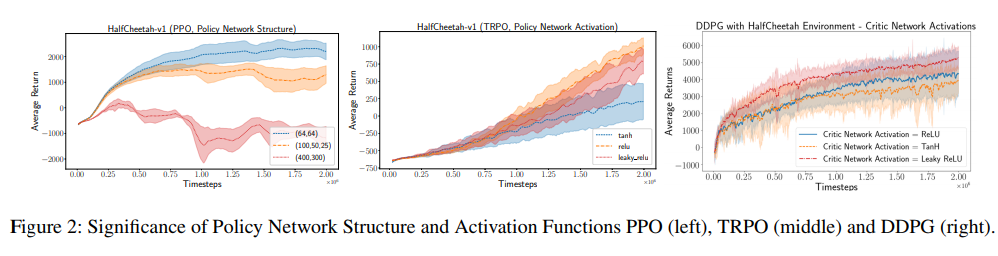
\includegraphics[width=1\columnwidth]{activation_functions.png}

    \item Changing random seed can end up with non-identical distributions from each cycle of running the experiment on the algorithms and that can be explained with the variance from one complete iteration to the other one.
    
    \item Sensitivity to hyperparametes and configuration of the environment and also algorithms can lead to far different outcomes and possibilities. Therefore bringing all of the factors under control is a decision making factor in either comparison or implementation of each of these algorithms.
 \end{itemize}




% This is an example citation \autocite{ginsberg}.
% \lipsum[1] % dummy text

% This is another example citation \autocite{brassard}.
% \lipsum[2] % dummy text

% This is a repeated citation \autocite{brassard}.
% \lipsum[3] % dummy text

% This is another example citation \autocite{adorf}.
% \lipsum[4] % dummy text 

\end{document}